\documentclass{beamer} %

%%%BASICS
\usepackage[utf8]{inputenc}
\usepackage{csquotes}
\usepackage{physics}
\usepackage{tikz}
\usepackage{hyperref}
\usepackage{soul}
\usetikzlibrary{quantikz}
%%%START THEME SETTINGS
\usetheme{Dresden}
\usecolortheme{beaver}
\usefonttheme{professionalfonts}
\setbeamertemplate{itemize item}{\color{red}$\blacksquare$}
%%%END THEME SETTINGS

%%%START APA
\usepackage[british]{babel}
\usepackage[backend=biber,style=apa]{biblatex}
\DeclareLanguageMapping{british}{british-apa}
\addbibresource{references.bib}
%% APA citing
%% \cite{t} - Uthor und Richter, 2010
%% \textcite{t} - Uthor und Riter (2010)
%% \parencite{t} - (Uthor & Riter, 2010)
%% \parencite[Chapt.~4]{t} - (Uthor & Riter, 2010, S. 15)
%%%END APA



\title[CCP]{A unified picture of \\Balance puzzles and Group testing }
\institute[IITM]{Indian Institute of Technology Madras}
\author{Amrit Putcha, Siddhartha Chaganti}

\date{\today}

\begin{document}

\begin{frame}
	\titlepage
\end{frame}

%------------------------------------------------------
\begin{frame}
	\begin{block}{Testing (or querying) is a process to reveal or enhance a particular hidden feature of a specimen.}
		
	\end{block}
	\begin{center}
		
\includegraphics[scale = 0.4]{Figures/amrit1.png}
	\end{center}
\end{frame}
\begin{frame}
	\begin{block}{Naive way would be to weigh each specimen individually. But we can do better.}
		
	\end{block}
	\begin{center}
		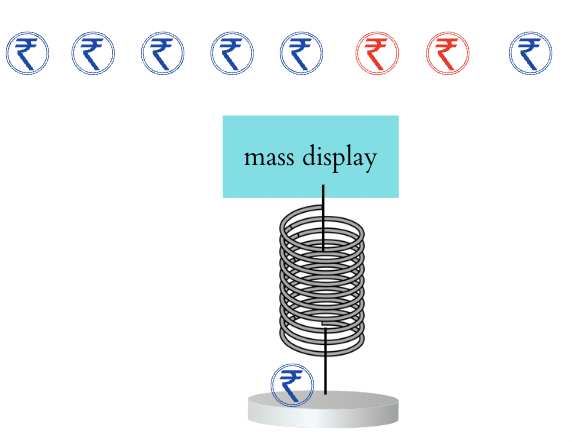
\includegraphics[scale = 0.5]{Figures/amrit2.png}
	\end{center}
\end{frame}
\begin{frame}
	\begin{block}{Group Testing}
		
	\end{block}
	\begin{center}
		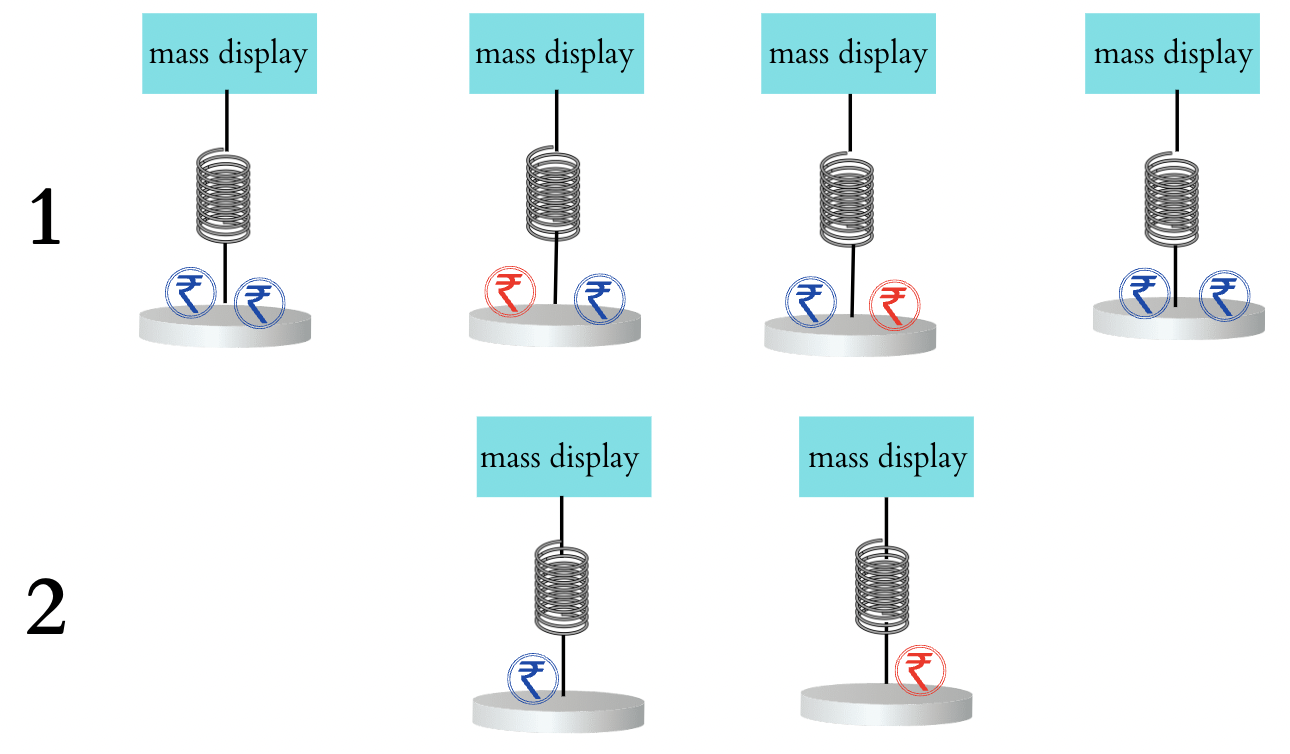
\includegraphics[scale = 0.4]{Figures/amrit3.png}
	\end{center}
\end{frame}
\begin{frame}
	\begin{block}{Li's S stage algorithm}
		\begin{itemize}
			\item For S=1, the number of queries required are N, where N is the total number of specimens. 
			\item For S=2, g1 groups of size k1 in stage 1 and g2 groups of size k2 in stage 2 and so on.
		\end{itemize}
		
	\end{block}
	\begin{center}
		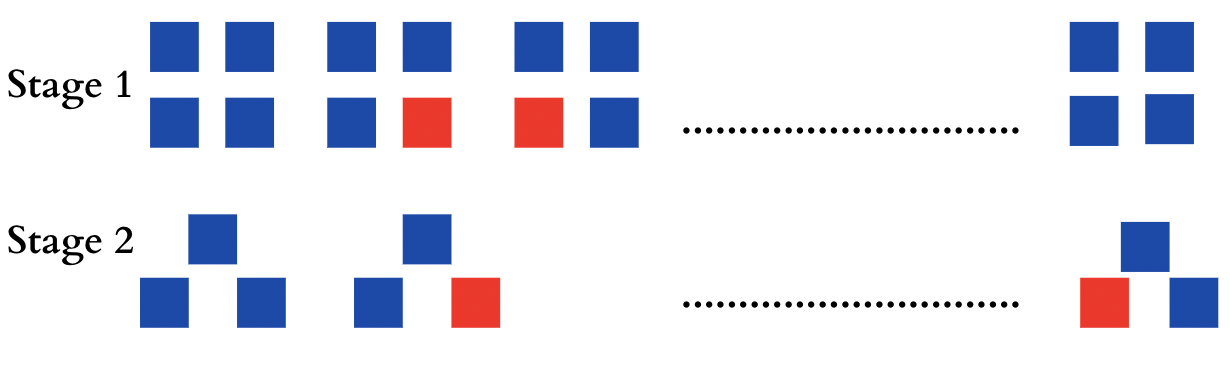
\includegraphics[scale = 0.4]{Figures/amrit4.png}
	\end{center}
\end{frame}
\begin{frame}
	\begin{block}{The Math}
		Calculations show that for S=2, the tests in the worst case scenario come out to be
		\[
			t_2 = g_2 + g_1 \leq \frac{n}{k_1} + d k_1
		\]
		Upper bound is minimized by \(k_1 = \sqrt{\frac{n}{d}} \) 
		\[
			\text{This gives us } g_1 = \sqrt{nd} \& t_2 \leq 2\sqrt{nd} 
		\]
		Similar calculations are performed for S stages and the maximum number of tests comes out to be 
		\[
			t_s \leq sd\left(\frac{n}{d}\right)^\frac{1}{s} \leq ed \ln \left(\frac{n}{d}\right)
		\]
	\end{block}
\end{frame}
	
	\begin{frame}
		\begin{block}{Cases of Concern}
			The pooling strategy discussed may not be optimal when the prevalence rate
				'p' is above certain threshold.  p = d/N should be less than 1.\\
			Thus for S=2,  p should be less than 0.25, otherwise the number of tests become
				more than the population size, and the activity becomes useless.\\
			Similarly, a threshold value for the prevalence rate can be calculated for S stages
				and it comes out to satisfy   
				\[
					-p \ln (p) \geq \frac{1}{e}
				\]
				
				
		\end{block}
	\end{frame}
	\begin{frame}
		\begin{block}{Problem Statement}
			N similar specimens from suspected patients and a test for the presence of the infection, d are infected.
		\end{block}
		
\includegraphics[scale = 0.5]{Figures/amrit5.png}
		\begin{block}{}
			What is the maximum tests required by the Li's pooling strategy considering 'g' pools of size 'k' ?
		\end{block}
	\end{frame}
	\begin{frame}
		\begin{block}{Deutsch-Josza Algorithm}
			Given a boolean function \(f\), which takes as input a string of bits, and returns either 0 or 1, 
			\[
				f : \{x_1,x_2\dots\} \to 0 \text{ or }  1 , \text{ where $x_n$ is 0 or 1. } 
			\]
			The property of the given Boolean function is that it is guaranteed to either be balanced or constant. Our task is to determine whether the given function is balanced or constant.
		\end{block}
		\begin{center}
			\begin{quantikz}[slice all]
				\lstick{\(\ket{0}^{\otimes n}\)}&[2mm]\gate{H^{\otimes n}}\qwbundle{n}&\gate[wires=2][1.7cm]{\textsc{\(U_f\) } }\gateinput{\(x\)}\gateoutput{\(x\)}&\gate{H^{\otimes n}}&\meter{}&\qw\\
				\lstick{\(\ket{1}\)}&[2mm]\gate{H}&\qw\gateinput{\(y\)} \gateoutput{\(y\oplus f(x)\)}&\qw&\qw&\qw
			\end{quantikz}	
		\end{center}
		
	\end{frame}
	\begin{frame}
		\begin{block}{Bernstein-Vazirani Algorithm}
			Given a boolean function \(f\), which takes as input a string of bits, and returns either 0 or 1, 
			\[
				f : \{x_1,x_2\dots\} \to 0 \text{ or }  1 , \text{ where $x_n$ is 0 or 1. } 
			\]
			the function is guaranteed to return the bitwise product of the input with some string,s . 
			In other words, given an input \(x\), \(f(x) = s. x \mod 2\). We are expected to find s. 
				 
		\end{block}
		\begin{center}
			\begin{quantikz}[slice all]
				\lstick{\(\ket{0}^{\otimes n}\)}&[2mm]\gate{H^{\otimes n}}\qwbundle{n}&\gate[wires=2][3cm]{\textsc{\(Q_s\) } }\gateinput{\(x\)}\gateoutput{\(x\)}&\gate{H^{\otimes n}}&\qw\\
				\lstick{\(\ket{1}\)}&[2mm]\gate{H}&\qw\gateinput{\(y\)} \gateoutput{\(y\oplus s .  x \text{ mod 2}\)}&\qw&\qw
			\end{quantikz}
		\end{center}
	\end{frame}
	\begin{frame}
		\begin{block}{Quantum Solution to Bernstein-Vazirani Algorithm}
			\begin{enumerate}
				\item Initialize the qubits to the \( \ket{0}^{\otimes n}\) state, and the output qubit to \(\ket{-}\) state. 
				\item Apply Hadamard gates to input register. 
				\item Query the oracle. 
				\item Apply the Hadamard gates to the input register. 
				\item Measure. 
			\end{enumerate}
				 
		\end{block}
		\begin{center}
			\begin{quantikz}[slice all]
				\lstick{\(\ket{0}^{\otimes n}\)}&[2mm]\gate{H^{\otimes n}}\qwbundle{n}&\gate[wires=2][3cm]{\textsc{\(Q_s\) } }\gateinput{\(x\)}\gateoutput{\(x\)}&\gate{H^{\otimes n}}&\qw\\
				\lstick{\(\ket{1}\)}&[2mm]\gate{H}&\qw\gateinput{\(y\)} \gateoutput{\(y\oplus s .  x \text{ mod 2}\)}&\qw&\qw
			\end{quantikz}
		\end{center}
	\end{frame}
	\begin{frame}
		\begin{block}{RTPCR/ Counterfeit Coin problem as Bernstein Vazirani problem}
			\begin{itemize}
				\item The word sample is used to represent RT-PCR sample and Coin. 
				\item If a sample is tested then we represent the qubit respective to it as \(\ket{1}\) else \(\ket{0}\). 
				\item The oracle contains wether the sample is different from others or not. (which is unknown to us.)
				\item By above method we can clearly convert our problem of sample testing to Bernstein Vazirani problem.
			\end{itemize}
		\end{block}
	\end{frame}
	\begin{frame}
		\begin{block}{Circuit for Sample testing with sample size 8}
			
		\end{block}
		\begin{center}
			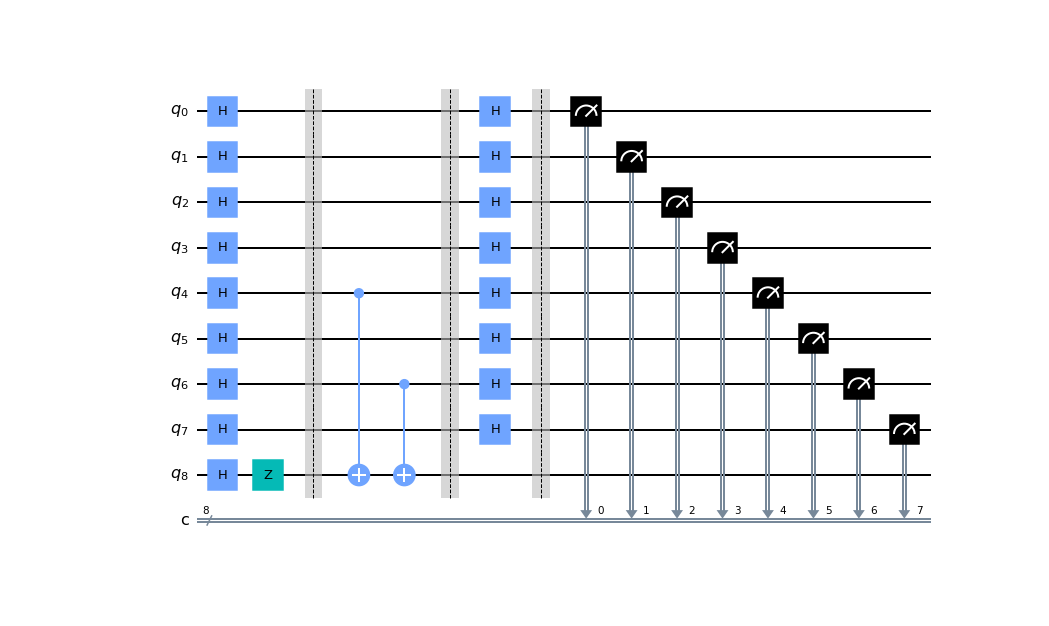
\includegraphics[scale = 0.3]{Figures/circuit-8.png}
		\end{center}
	\end{frame}
	\begin{frame}
		\begin{block}{Result on qsam simulator for sample size of 8}
			
		\end{block}
		\begin{center}
			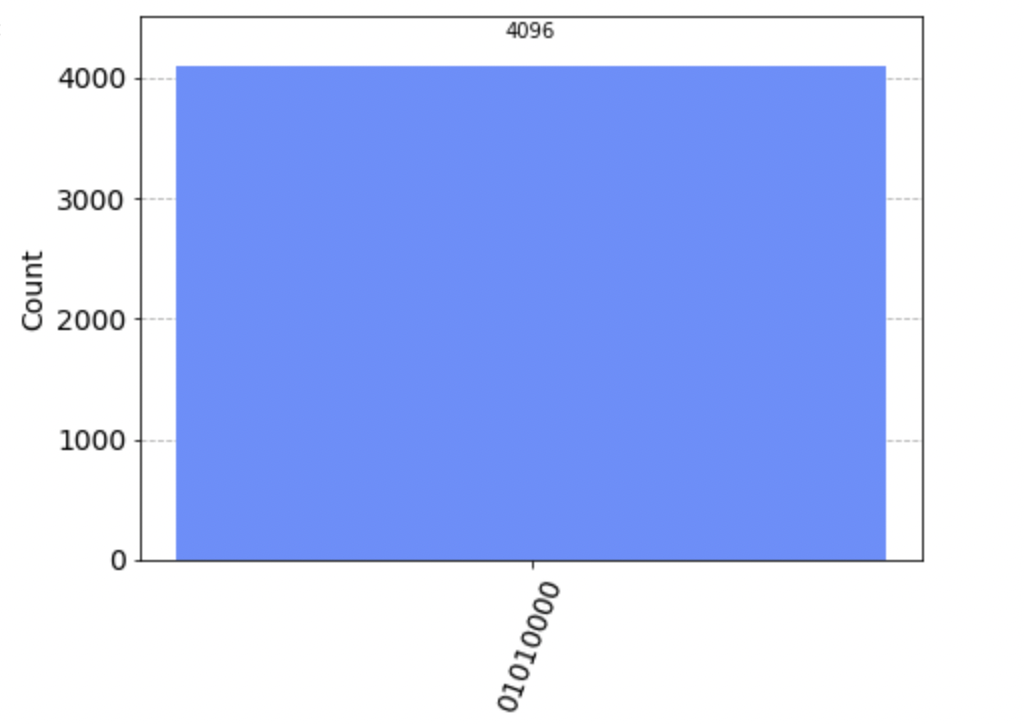
\includegraphics[scale = 0.5]{Figures/histogram-8.png}
		\end{center}
	\end{frame}
		\begin{frame}
			\begin{block}{Circuit for Sample testing with sample size 5}
				
			\end{block}
			\begin{center}
				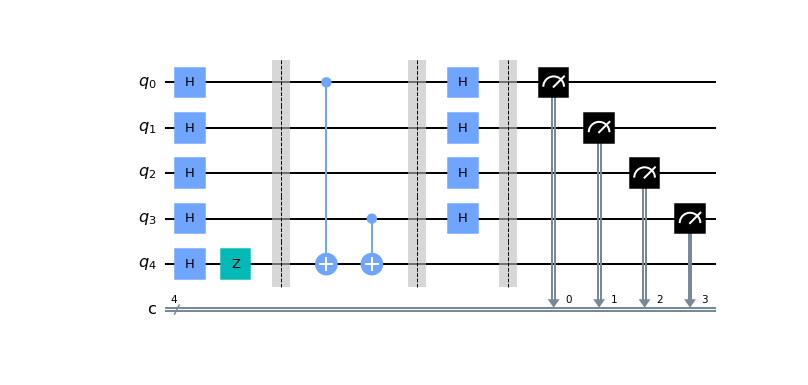
\includegraphics[scale = 0.4]{Figures/circuit-5 qubit.png}
			\end{center}
		\end{frame}
		\begin{frame}
			\begin{block}{Transpiled circuit}
				
			\end{block}
			\begin{center}
				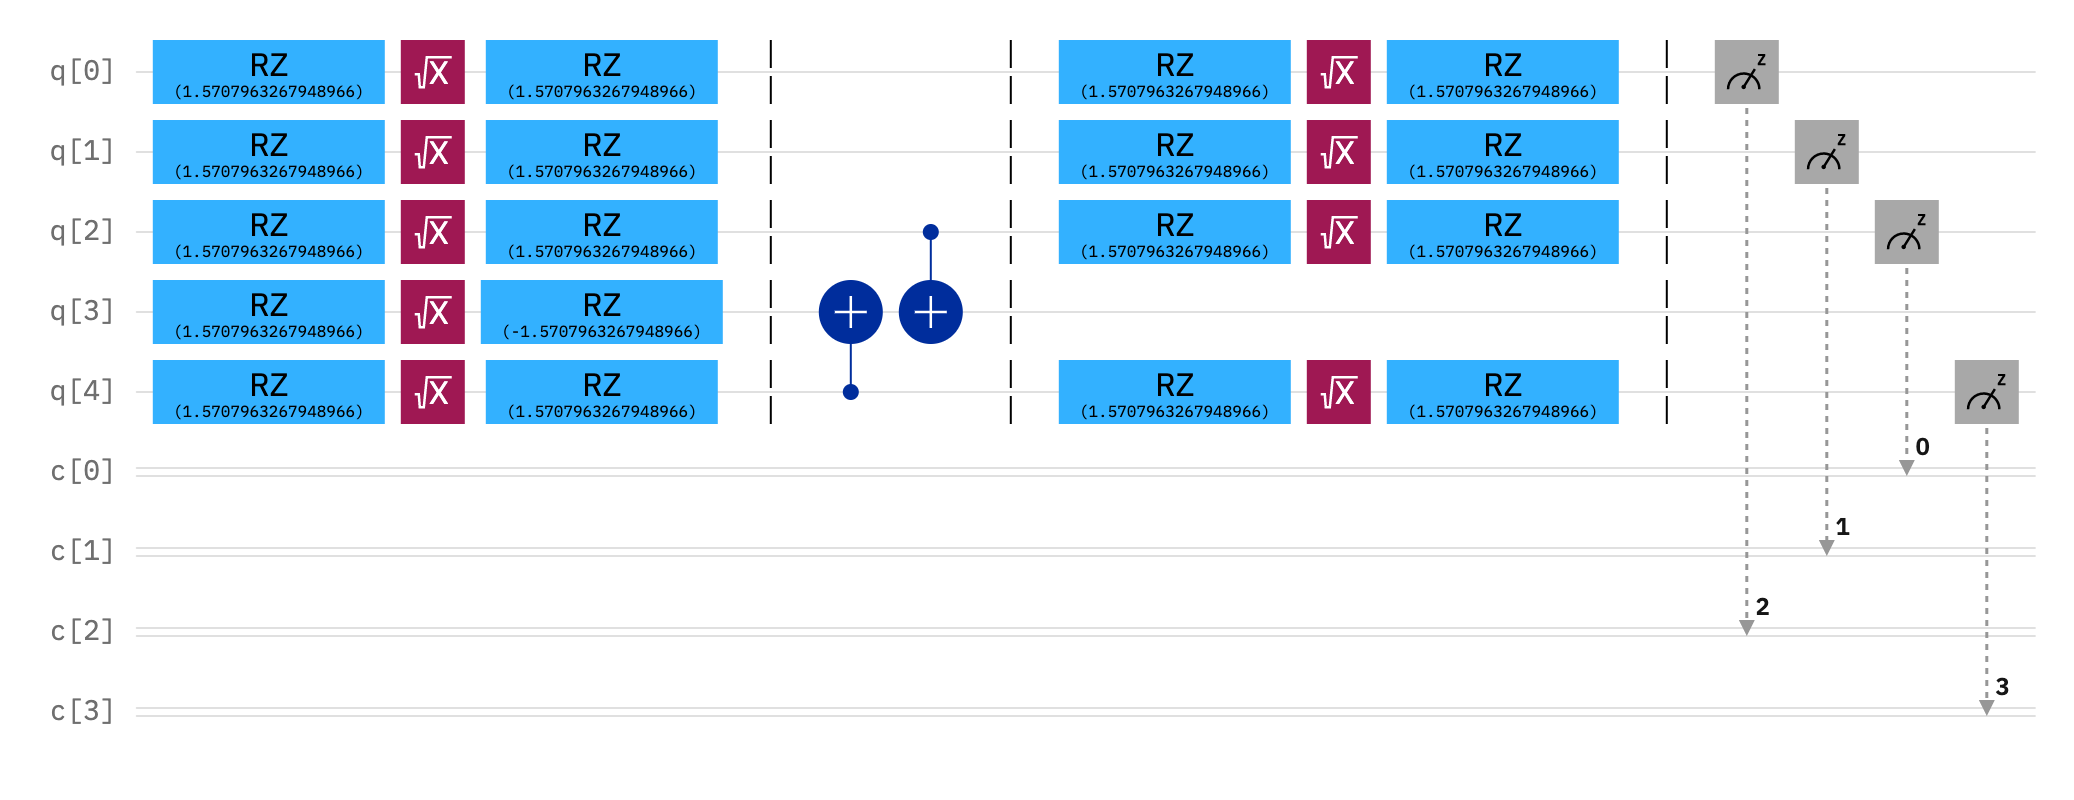
\includegraphics[scale = 0.1]{Figures/transpiled-circuit.png}
			\end{center}
			
		\end{frame}
		\begin{frame}
			\begin{block}{Result ibmq  machine for sample size 5}
				
			\end{block}
			\begin{center}
				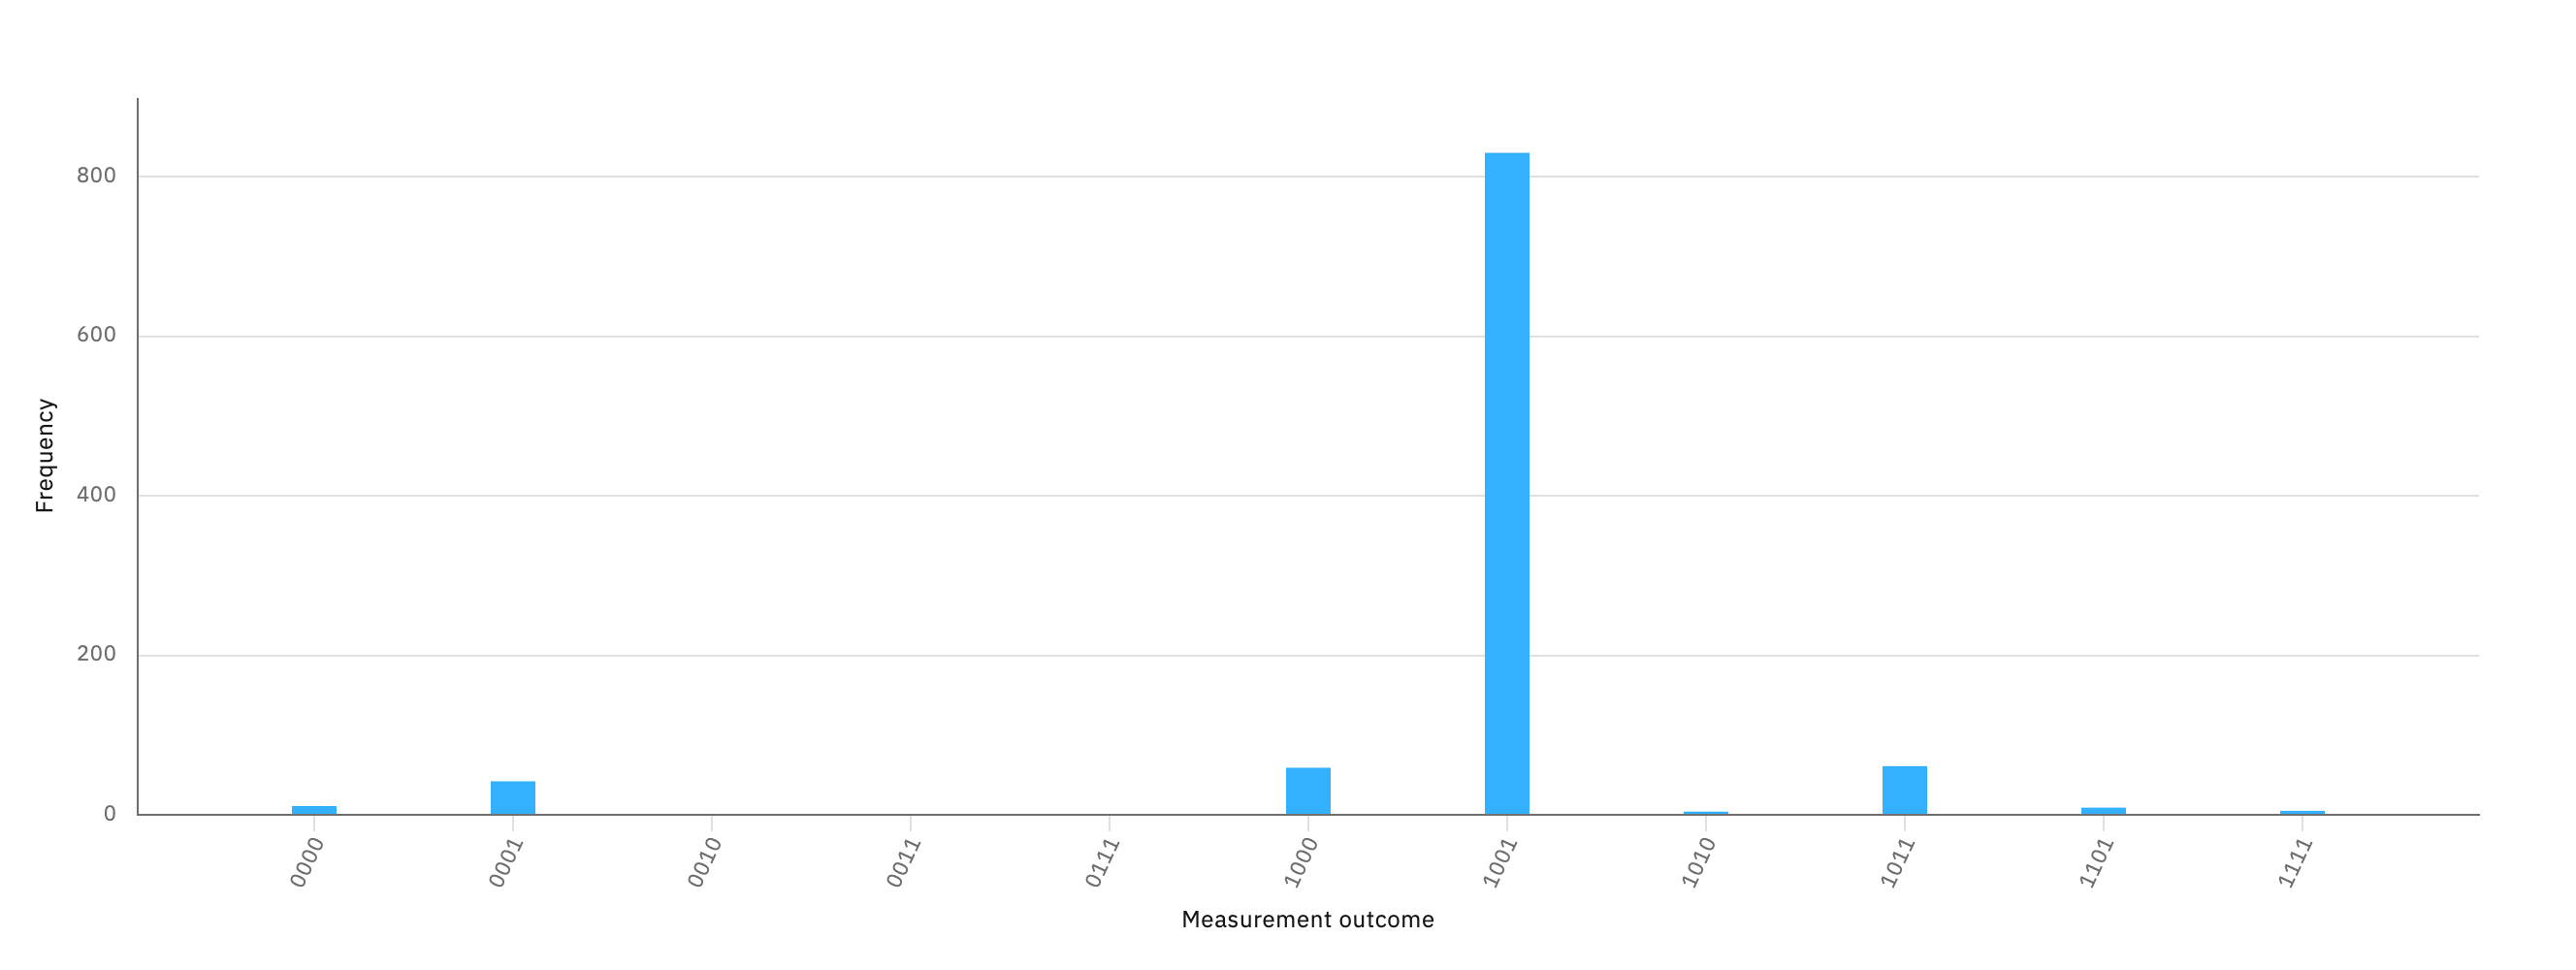
\includegraphics[scale = 0.1]{Figures/ibm_hist.png}
			\end{center}
	\end{frame}
	\begin{frame}
		\begin{block}{Future scope}
			In the past Iwama et.al4 has considered solving the balance puzzle using quantum mechanics. They have aptly named it the ”quan- tum counterfeit coin” puzzle. They however in their article consider a beam balance rather than a spring balance. Due to this they consider a query trit (ternary bit) string rather than a query bit string. A single trit is considered to be of a value either ’-1’,’0’ or ’1’. -1 representing placing the coin on left pan, 1 representing placing on the right pan and 0 placing it nowhere. Moreover, the Hamming weight of the query string in their case has to be even (i.e. the number of trits in the trit string different than 0 has to be even).
		\end{block}
	\end{frame}
	\begin{frame}
		\begin{block}{References}
			\begin{itemize}
				\item A unified picture of Balance puzzles and Group testing : Some lessons from quantum mechanics for the pandemic. Chetan Waghela. 
				\item Kazuo Iwama, Harumichi Nishimura, Rudy Raymond, and Junichi Teruyama\\
				Quantum Counterfeit Coin Problems.\\
				In Proceedings of 21st International\\ Symposium on Algorithms and Computation (ISAAC2010), LNCS 6506, pp.73-84, 2010.
				arXiv:1009.0416
				
			\end{itemize}
		\end{block}
	\end{frame}
\end{document}
